\section{Visualisations - Conditions aux limites réflectives}

Les figures ci-dessous montrent la magnitude du champ électromagnétique
et la distribution de la chaleur dans l'enceinte du four avec l'aliment
dedans.

La source du champ magnétique se trouve à gauche dans toutes les
figures. Voir les sections~\ref{experiences_numeriques:constantes}
et~\ref{experiences_numeriques:dimensions_four} pour consulter
les valeurs des paramètres physiques et les dimensions du four.


\begin{figure}[H]
    \centering
    \begin{subfigure}{.5\textwidth}
        \centering
        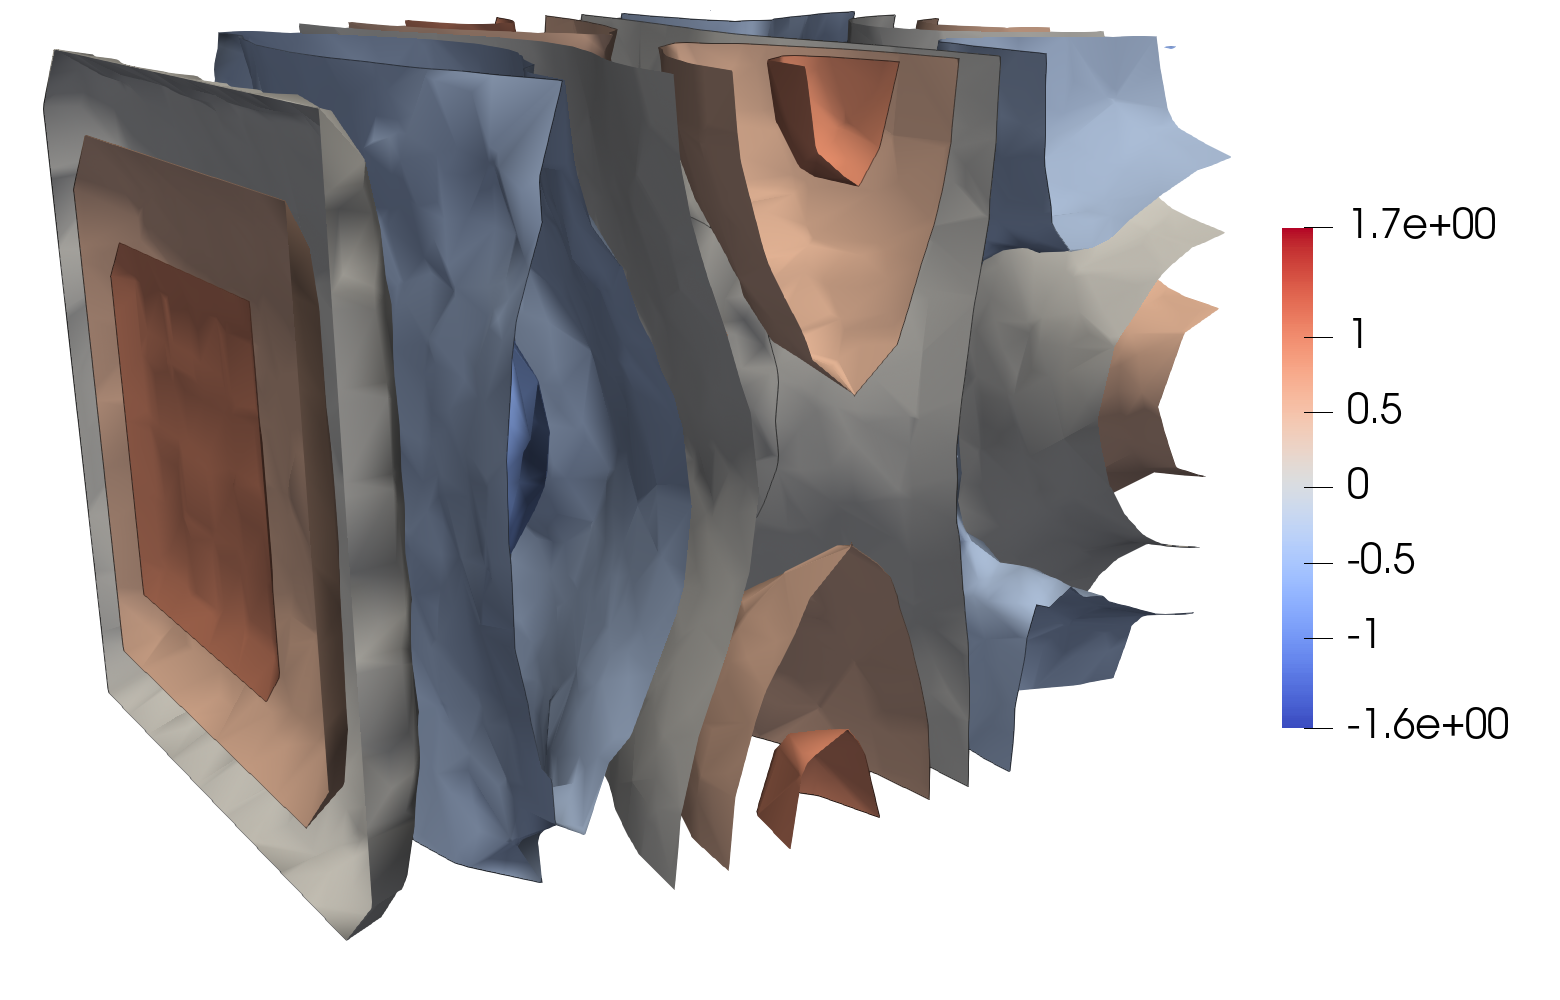
\includegraphics[scale=0.15]{figures/helmholtz/helmholtz_reel_reflexion1.png}
        \caption{Partie réelle}
    \end{subfigure}%
    \begin{subfigure}{.5\textwidth}
        \centering
        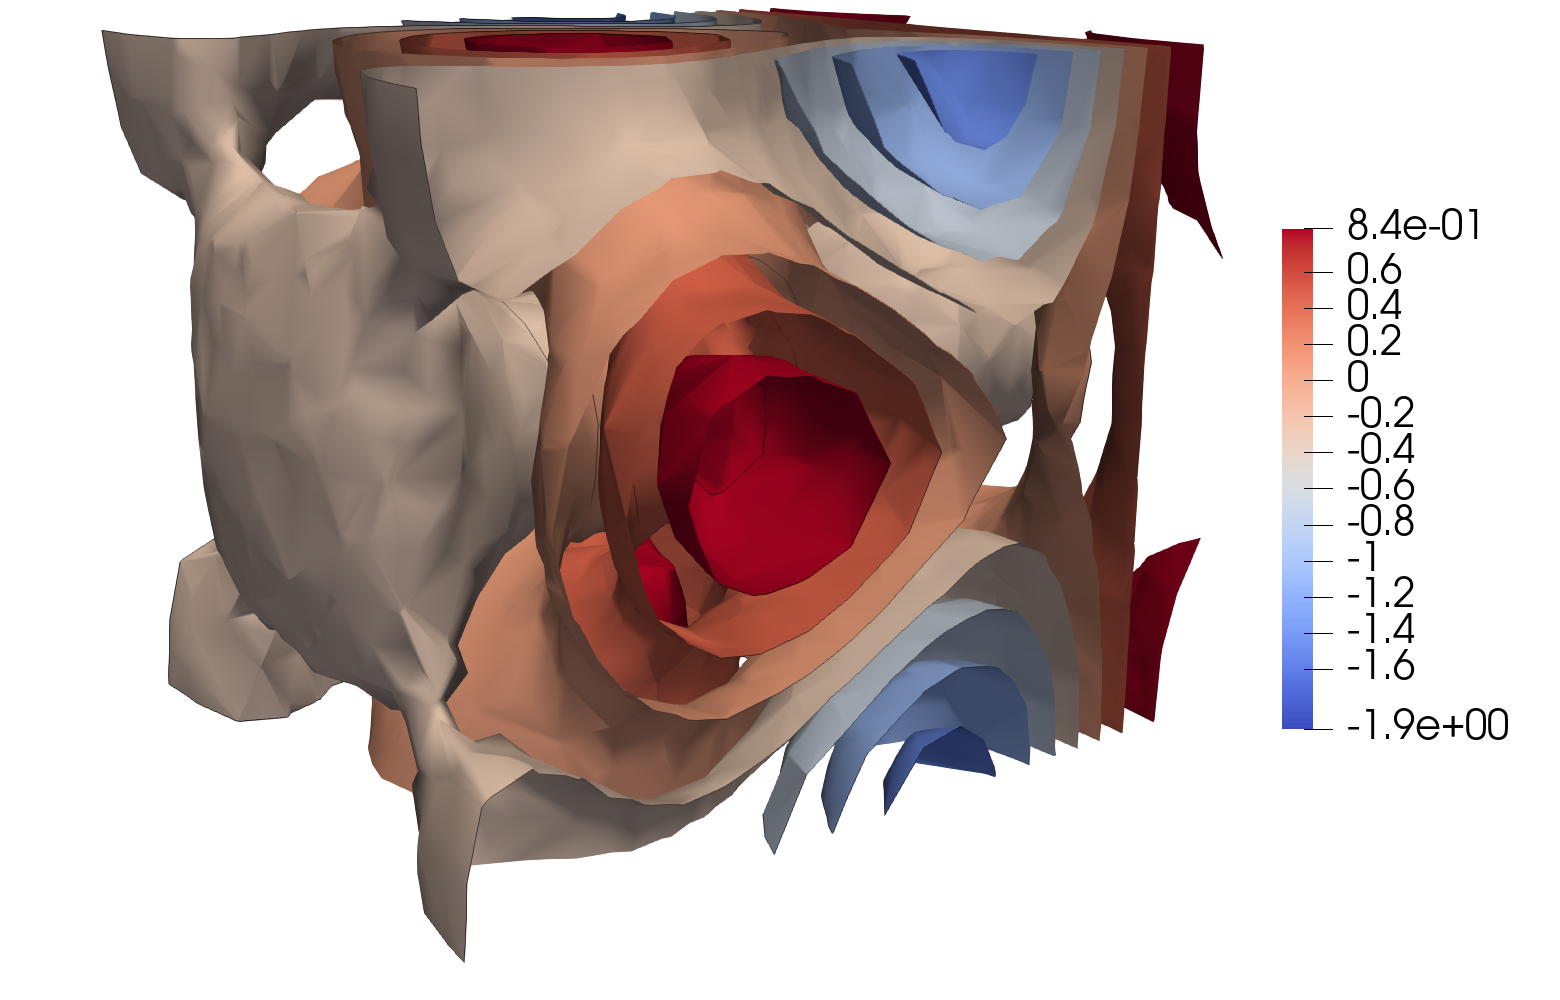
\includegraphics[scale=0.15]{figures/helmholtz/helmholtz_imag_reflexion1.png}
        \caption{Partie imaginaire}
    \end{subfigure}
    \caption{Des tracés de contours de la magnitude du champ électromagnétique
    dans l'enceinte du four avec l'aliment dedans.}
\end{figure}

\begin{figure}[H]
    \centering
    \begin{subfigure}{.5\textwidth}
        \centering
        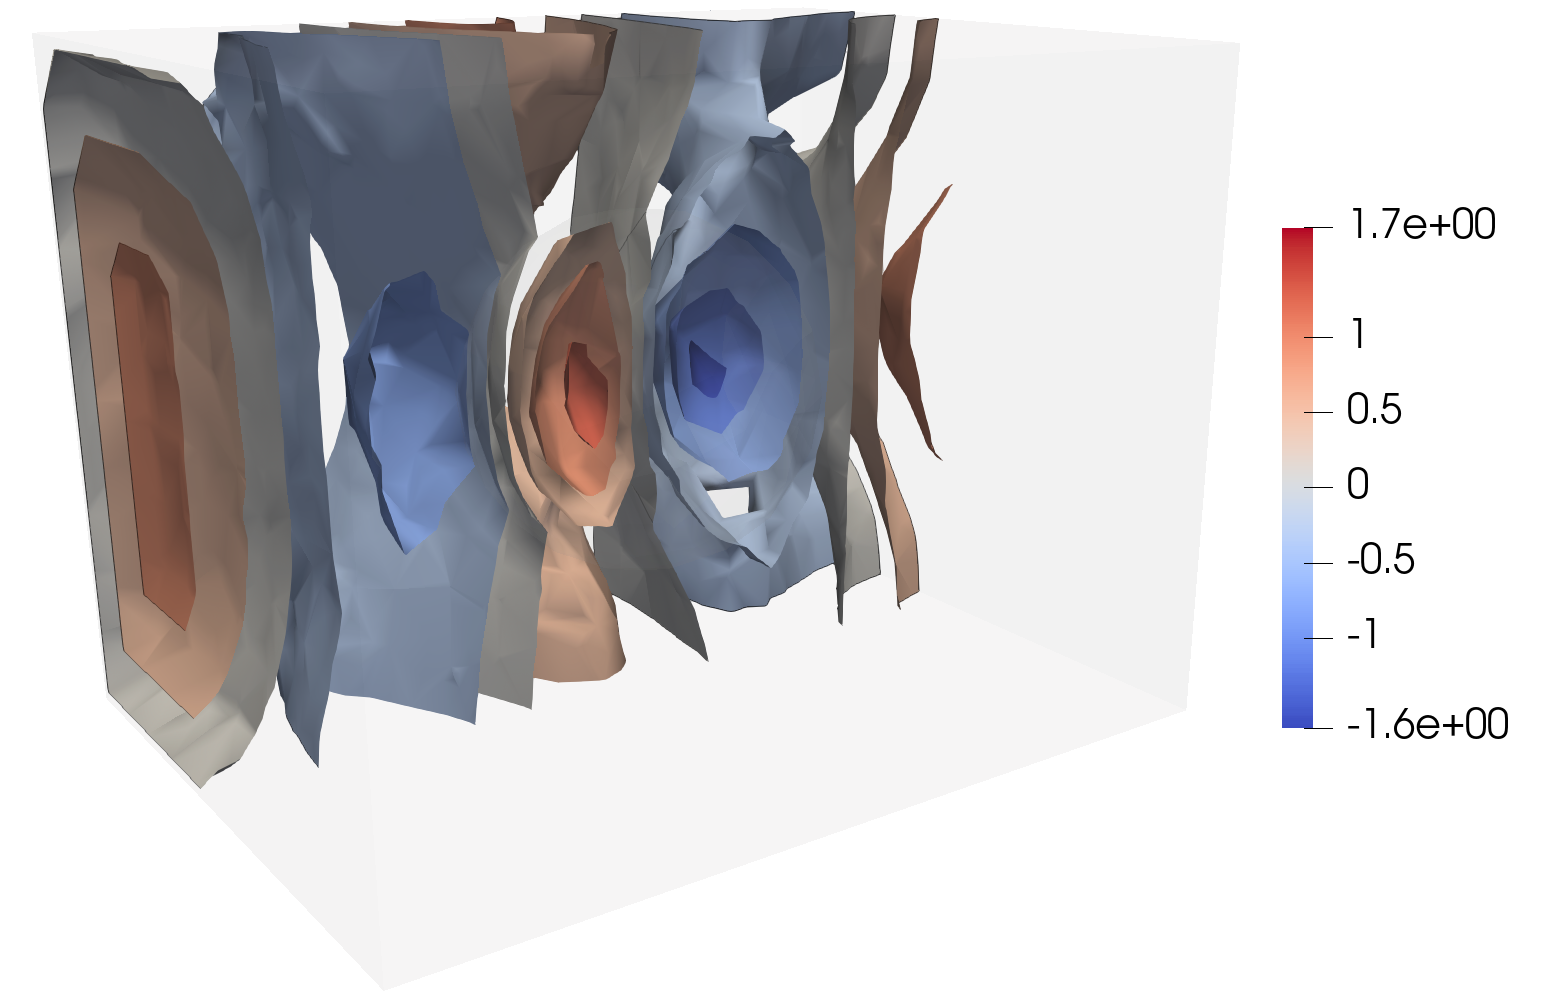
\includegraphics[scale=0.15]{figures/helmholtz/helmholtz_reel_reflexion2.png}
        \caption{Partie réelle}
    \end{subfigure}%
    \begin{subfigure}{.5\textwidth}
        \centering
        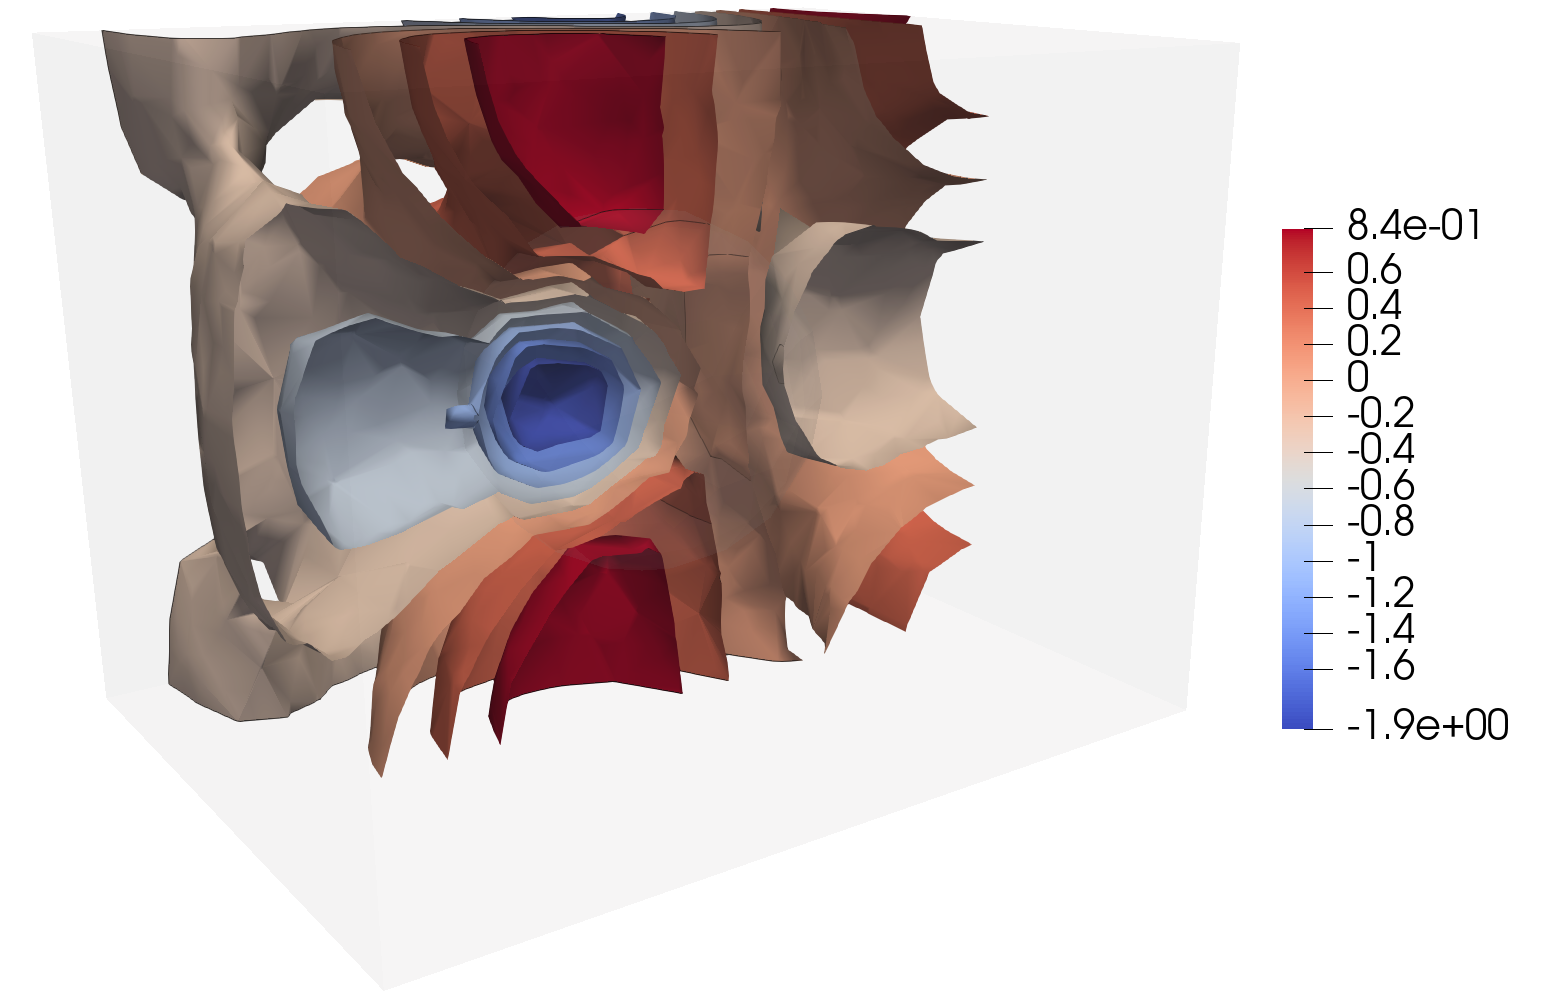
\includegraphics[scale=0.15]{figures/helmholtz/helmholtz_imag_reflexion2.png}
        \caption{Partie imaginaire}
    \end{subfigure}
    \caption{Des clips des tracés de contours de la magnitude du champ
    électromagnétique dans l'enceinte du four avec l'aliment dedans.
    Le clip est au milieu du four dans le plan $x\text{-}y$.}
\end{figure}

\begin{figure}[H]
    \centering
    \begin{subfigure}{.5\textwidth}
        \centering
        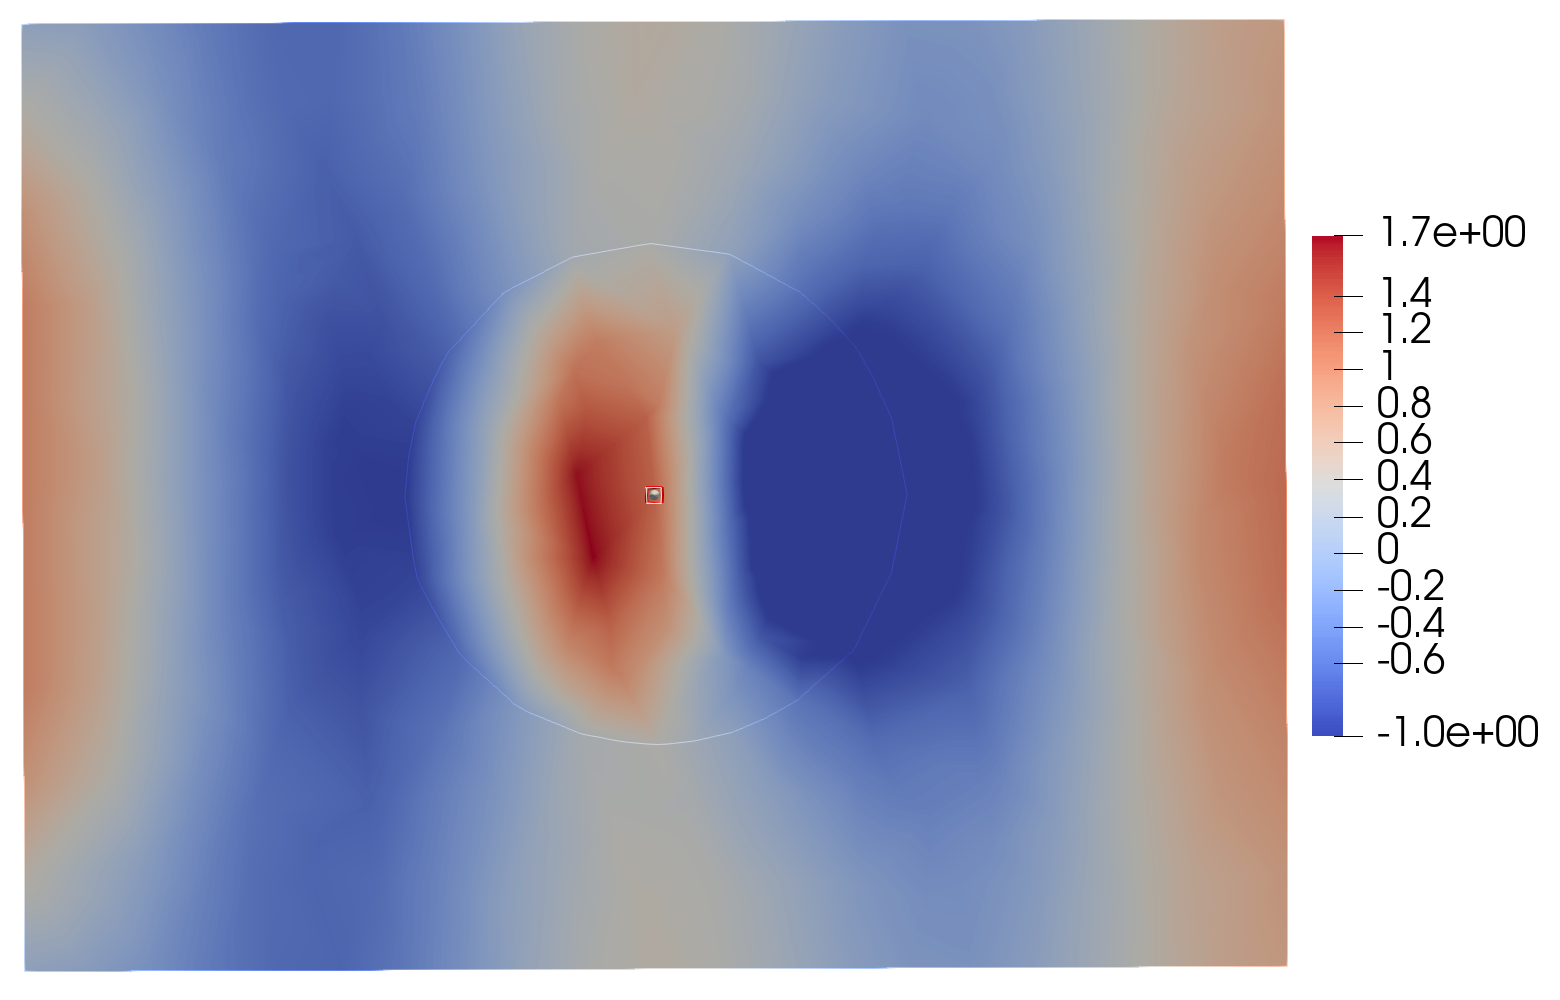
\includegraphics[scale=0.15]{figures/helmholtz/helmholtz_reel_reflexion3.png}
        \caption{Champ réel}
    \end{subfigure}%
    \begin{subfigure}{.5\textwidth}
        \centering
        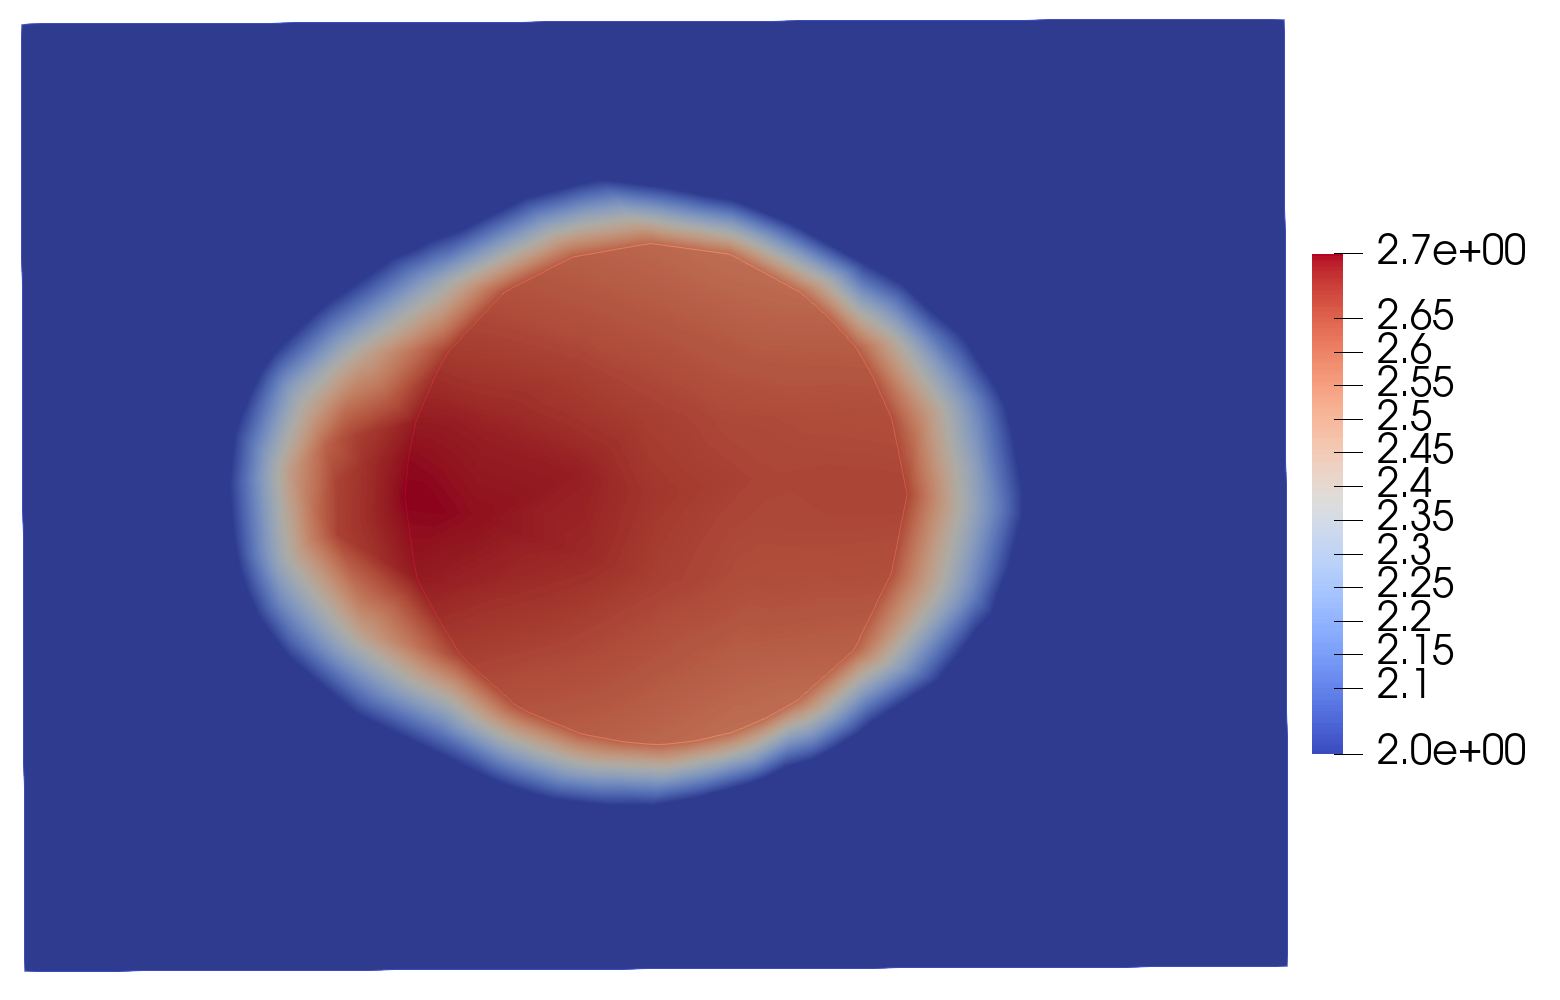
\includegraphics[scale=0.15]{figures/chaleur/chaleur_reflexion1.png}
        \caption{Chaleur}
    \end{subfigure}
    \caption{Des tranches de la partie réelle de la magnitude du champ
    électromagnétique et la chaleur dans l'enceinte du four avec
    l'aliment dedans. La tranche est orientée selon l'axe $x$.}
\end{figure}
